
\begin{figure*}
	\centering
	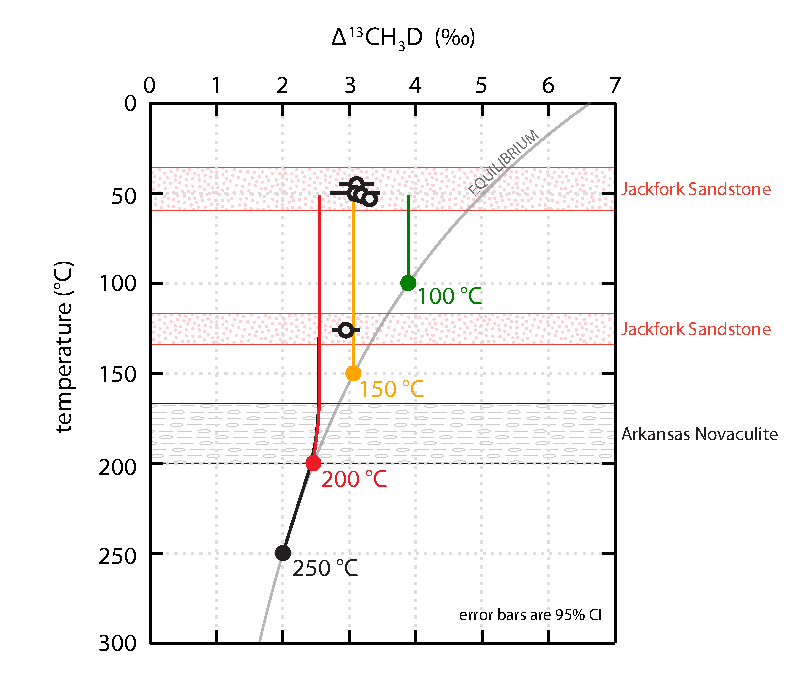
\includegraphics[width=0.9\textwidth]{figures/FigA.4.pdf}
%	\captionsetup{format=myformat}	% hrule beneath caption
	\caption[Cooling model for migrated gases at Potato Hills]{Model of migrating gases. The colored points on the
		model curves represent initial compositions of natural gases that were
		generated at 350~Ma at temperatures from 100 to 250~°C. The gases were
		assumed to be carrying Δ\textsuperscript{13}CH\textsubscript{3}D values
		equal to those expected for equilibrium at these starting temperatures.
		These model gases then were cooled at a rate of 10~°C per Myr until 330~Ma, at which cooling ceased. Curves show the predicted clumped
		isotopologue compositions of gases (\emph{x}-axis) with temperature (\emph{y}-axis).
		Clumped isotopologue reordering was treated as a first-order reaction
		obeying the Arrhenius equation, with pre-exponential factor
		\SI{6.1e9}{\second^{-1}} and activation energy
		209 kJ mol\textsuperscript{$-$1} \parencite[estimated from the data of][]{Koepp_1978}. Data from \autoref{tab:A:1} are shown for comparison. The equilibrium
		curve is that of \textcite{Wang++_2015_S}, for which the equation is listed in
		\autoref{dx:C} (\autoref{eqn:C:equilibrium}).}
	\label{fig:A:4}
\end{figure*}
